\chapter{Tabela de Probabilidades - Distribuição t-Student}

\begin{figure}[h]
	\center
	\label{fig:tab-prob-t-student}
	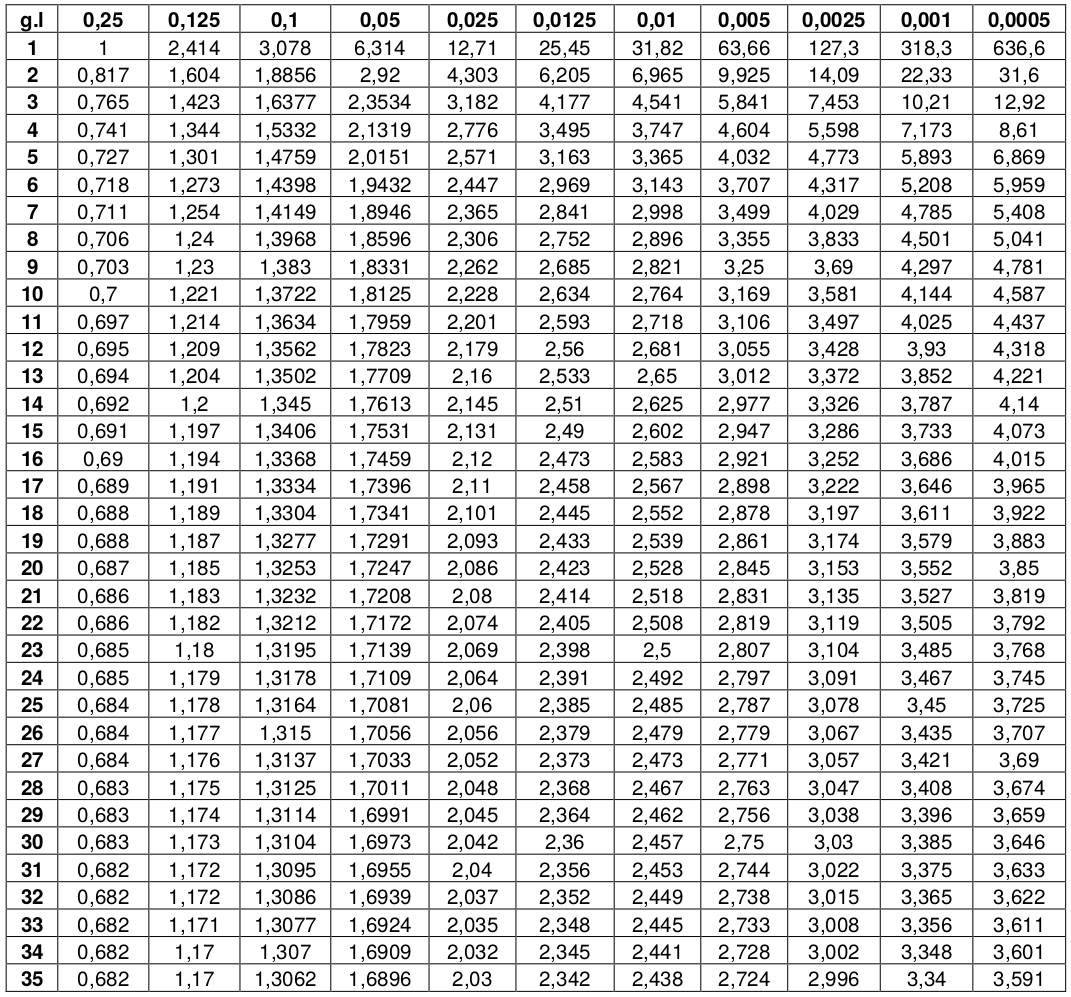
\includegraphics[scale=1.85]{apendices/prob-t-studend.png}
\end{figure}

Onde:
\begin{itemize}
	\item Os graus de liberdade \((n-1)\) estão no cabeçalho de linha;
	\item As probabilidades estão no cabeçalho de linha;	
	\item Os valores \(t\) estão no centro. 
\end{itemize}